\typeout{IJCAI-16 Instructions for Authors}
\documentclass{article}
\usepackage{times}
\usepackage{ijcai16}
\usepackage{times}
\usepackage{graphicx}
\usepackage{amsmath}
\usepackage{amsthm, amssymb}
\usepackage{enumerate}
\usepackage{fullpage}
\usepackage{hyperref}
\usepackage{soul}
\usepackage{xcolor}
\usepackage{float}
\usepackage{mathtools}
\usepackage{empheq}
\usepackage{comment}
\restylefloat{table}
\usepackage{listings}
\usepackage{color} %red, green, blue, yellow, cyan, magenta, black, white
\definecolor{mygreen}{RGB}{28,172,0} % color values Red, Green, Blue
\definecolor{mylilas}{RGB}{170,55,241}
\usepackage{fancybox}
\usepackage{framed}
\usepackage{mathrsfs}

\graphicspath{{Pictures/}}

\begin{document}
\title{Data Mining Corporate Emails to Model Employee Behaviors and Analyze Organizational Structure}
%\title{Organizational Relationship Classification From Data Mining Corporate Email Metadata}
\author{Kayla Straub\\
        Virginia Tech, Blacksburg, Virginia\\
        kstraub@vt.edu}
\maketitle

\begin{abstract}
\iffalse
Mine:
Organization charts do not always accurately reflect actual relationships within workplace.  This paper seeks to determine if true behaviors are instead exhibited in corporate email communication patterns.  Because the Enron dataset contained errors and lacked conclusive ground truth for employee titles, we turned to our own organization.  We collected and cleaned email metadata from volunteers in the center to build an original email database. From the email data, we calculated several features of two main types: traffic-based and social-graph-based. Using information gain, we evaluated which features were the best predictors of job title. This paper presents a thorough analysis of the features used and the random forest classifier we built to predict job titles with very high accuracy. In fact, correct labels could even be predicted for employees that did not volunteer in the study, but emailed frequently with those who had.  Finally, we compared connections in the email social graph to the official organization chart and found that email relationships do not consistently reflect the chain of command.

Joey's:
Email correspondence has become the predominant method of communication for businesses.  This electronically searchable data could be used to determine a lot about how employees interact if access to this data was not limited by serious privacy concerns. After the Enron dataset was made available, researchers were able to provide great insight based on the available data despite the many challenges with that dataset.  The work in this paper provides a suite of methods to be used on an appropriately anonymized email dataset.  This anonymized dataset from our internal email server is first used to validate classification algorithms and then to generate insight into the interactions within our center.  Analysis is performed on email metadata provided voluntarily by approximately half of the center.  This data is used to provide information not only about the participants, but also about the other members of the center with whom they are connected through their e-mails.  The result is a much fuller understanding of the center's operations than can be found in the official organization chart. 

Hybrid:
\fi
Email correspondence has become the predominant method of communication for businesses.  If not for the inherent privacy concerns, this electronically searchable data could be used to better understand how employees interact. For example, after the Enron dataset was made available, researchers were able to provide great insight into employee behaviors based on the available data despite the many challenges with that dataset.  The work in this paper demonstrates the application of a suite of methods to an appropriately anonymized email dataset created from volunteers' email metadata.  This new dataset, from an internal email server, is first used to validate machine learning and feature extraction algorithms and then to generate insight into the interactions within the center.  Based solely on email data, a random forest  modeled behavior patterns and accurately classified not only participants in the study but also other members of the center who were connected to participants through email.  Furthermore, the data revealed relationships not present in the formal operating structure.  The result is a much fuller understanding of the center's internal structure than can be found in the official organization chart.

\end{abstract}

\section{Introduction}
\begin{itemize}
\item Talk about applications of determining work structure from email behavior?
\item Why problem is important/hard/unsolved


Email is a pervasive medium for communication in modern society - particularly in the workplace.  In 2015, there were estimated over 2.6 billion email users, and it is projected that by the end of 2019, over one third of the global population will be using email.  In fact, the average business email sends or receives 112 emails per day, accounting for 54.7\% of worldwide email traffic \cite{radicati_emails_2015}. Retention of large email archives has become common practice with decreasing memory size and cost \cite{fisher_revisiting_2006}.  In that study, out of 600 employees at a high-tech company, the average employee had 28,660 emails stored in 133 folders which is a significant increase from 10 years earlier.  This trove of interesting information can be leveraged to analyze the relationships between coworkers.

\item Talk about what all the sections you'll talk about
\end{itemize}

\section{Related Works}
Email has been a common research topic over the past decade.  This is in part because  the Enron email dataset was released in 2004 \cite{klimt_introducing_2004}, allowing researchers access to a rich collection of real-world corporate emails.  This dataset has been extensively researched on topics including spam classification \cite{martin_analyzing_2005}, \cite{gaber_e-mail_2016}, \cite{shams_classifying_2013}; email categorization \cite{he_novel_2014}, \cite{keila_structure_2005}; and recipient prediction \cite{sofershtein_predicting_2015}, \cite{hu_towards_2012}.  However, there are known flaws and discrepancies with even the most recent versions of this dataset -- ranging from misspelled email addresses \cite{nordbo_data_2014} to duplicate emails \cite{waterman_big_2014}. In one of the most popular forms of the dataset, \cite{shetty_enron_2004}, the database includes 253,735 emails sent as ``CC'' and  253,713 emails sent as ``BCC''.  Further inspection reveals that emails sent as one type or the other were almost always mistakenly recorded as both.

The existing literature on analyzing social email behavior is mainly divided into two categories: feature-based and social-based \cite{tang_email_2013}.  Feature-based methods calculate statistics based only on email patterns while social-based methods extract information from representing the email traffic as a social graph.

Using features extracted from email metadata, \cite{yelupula_social_2008} was able to cluster levels of management at Enron. In addition to email traffic statistics, using features such as the presence of different email attachment types and the length of emails were shown to successfully categorize email behavior in \cite{martin_analyzing_2005}.

Relational ties can be modeled as a graph network where nodes represent people and edges represent interactions.  This is a useful model because many statistics can be calculated from the layout of a social graph \cite{wasserman_social_1994}.  A common metric that has been shown to indicate importance in a social graph is betweenness centrality, which comes in several different flavors, and was first developed by \cite{freeman_set_1977}.  Betweenness centrality is a measure of how many shortest paths in a graph travel over each node.  A node with high betweenness centrality in a social graph has been shown to represent a high degree of influence on other nodes.  As \cite{tyler_email_2003} shows, a betweenness centrality algorithm can be used on a social graph to determine community structures within an organization.  However, other metrics have been used successfully as well.  For example, \cite{wilson_discovery_2009} detected the most important email users within a corporate network without using betweenness as a feature.  Instead, they used: degree, the number of edges connected to a node; density, the ratio of actual edges to the number of possible edges; and proximity prestige, the ratio of nodes that can reach a node $i$ to the average distance from those nodes to $i$.

Some research has been done in trying to combine the two different types of features.  An example of this approach is seen in \cite{rowe_automated_2007}, which combined features such as number of emails, response time, cliques, and degree centrality into a ``Social Score'' which was used to rank Enron employees.  The purpose of this paper is to further unite the two branches of research by aggregating old and novel email traffic statistics with social graph features and applying them to an original, clean dataset.

\begin{itemize}
\item Maybe add paragraph about algorithm-specific learning?
\end{itemize}

\section{Data Collection}
\begin{itemize}
\item Motivation for new data set
    \begin{itemize}
    \item No ground truth hierarchy for Enron
    \item Intimate knowledge of lab hierarchy/structure and personal interactions
    \end{itemize}
\item Anonymization process
\item First (37) vs. second ring (32) subjects for a total of 69 employees analyzed
    \begin{itemize}
    \item The first ring consisted of participants who signed release forms to collect metadata
    \item The second ring consisted of employees who did not sign a release form, but had known affiliation with the lab.  We also ensured that there were at least 100 emails in the database for each of these employees.
    \end{itemize}
\item Statistics
    \begin{itemize}
    \item Data collected
        \begin{itemize}
        \item Destination and source email address
        \item Email timestamp
        \item Subject prefix (if any)
        \item Hash of subject after removing prefix
        \item Hash of body text
        \item Length of subject in characters
        \item Length of body text in characters
        \item Whether email was encrypted/signed
        \end{itemize}
    \item Number of people (32118 distinct email addresses)
    \item Number of emails (2,276,770 in recipients table)
    \item Time period (1114 days/3.05 years, from 11/6/12-11/25/15(ish))
    \end{itemize}
\end{itemize}

\section{Features}
\begin{itemize}
\item Tried 102 different features: 70 traffic-based, 32 graph-based - briefly cover each (try to cite as much as you can!)
\item Briefly talk about ranker
\end{itemize}
\subsection{Traffic-Based Features}
\begin{itemize}
\item Highlight top 3 traffic-based features
\end{itemize}
\subsection{Social Network Features}
\begin{itemize}
\item Talk about how social graphs were created
\begin{figure}[H]
    \centering
        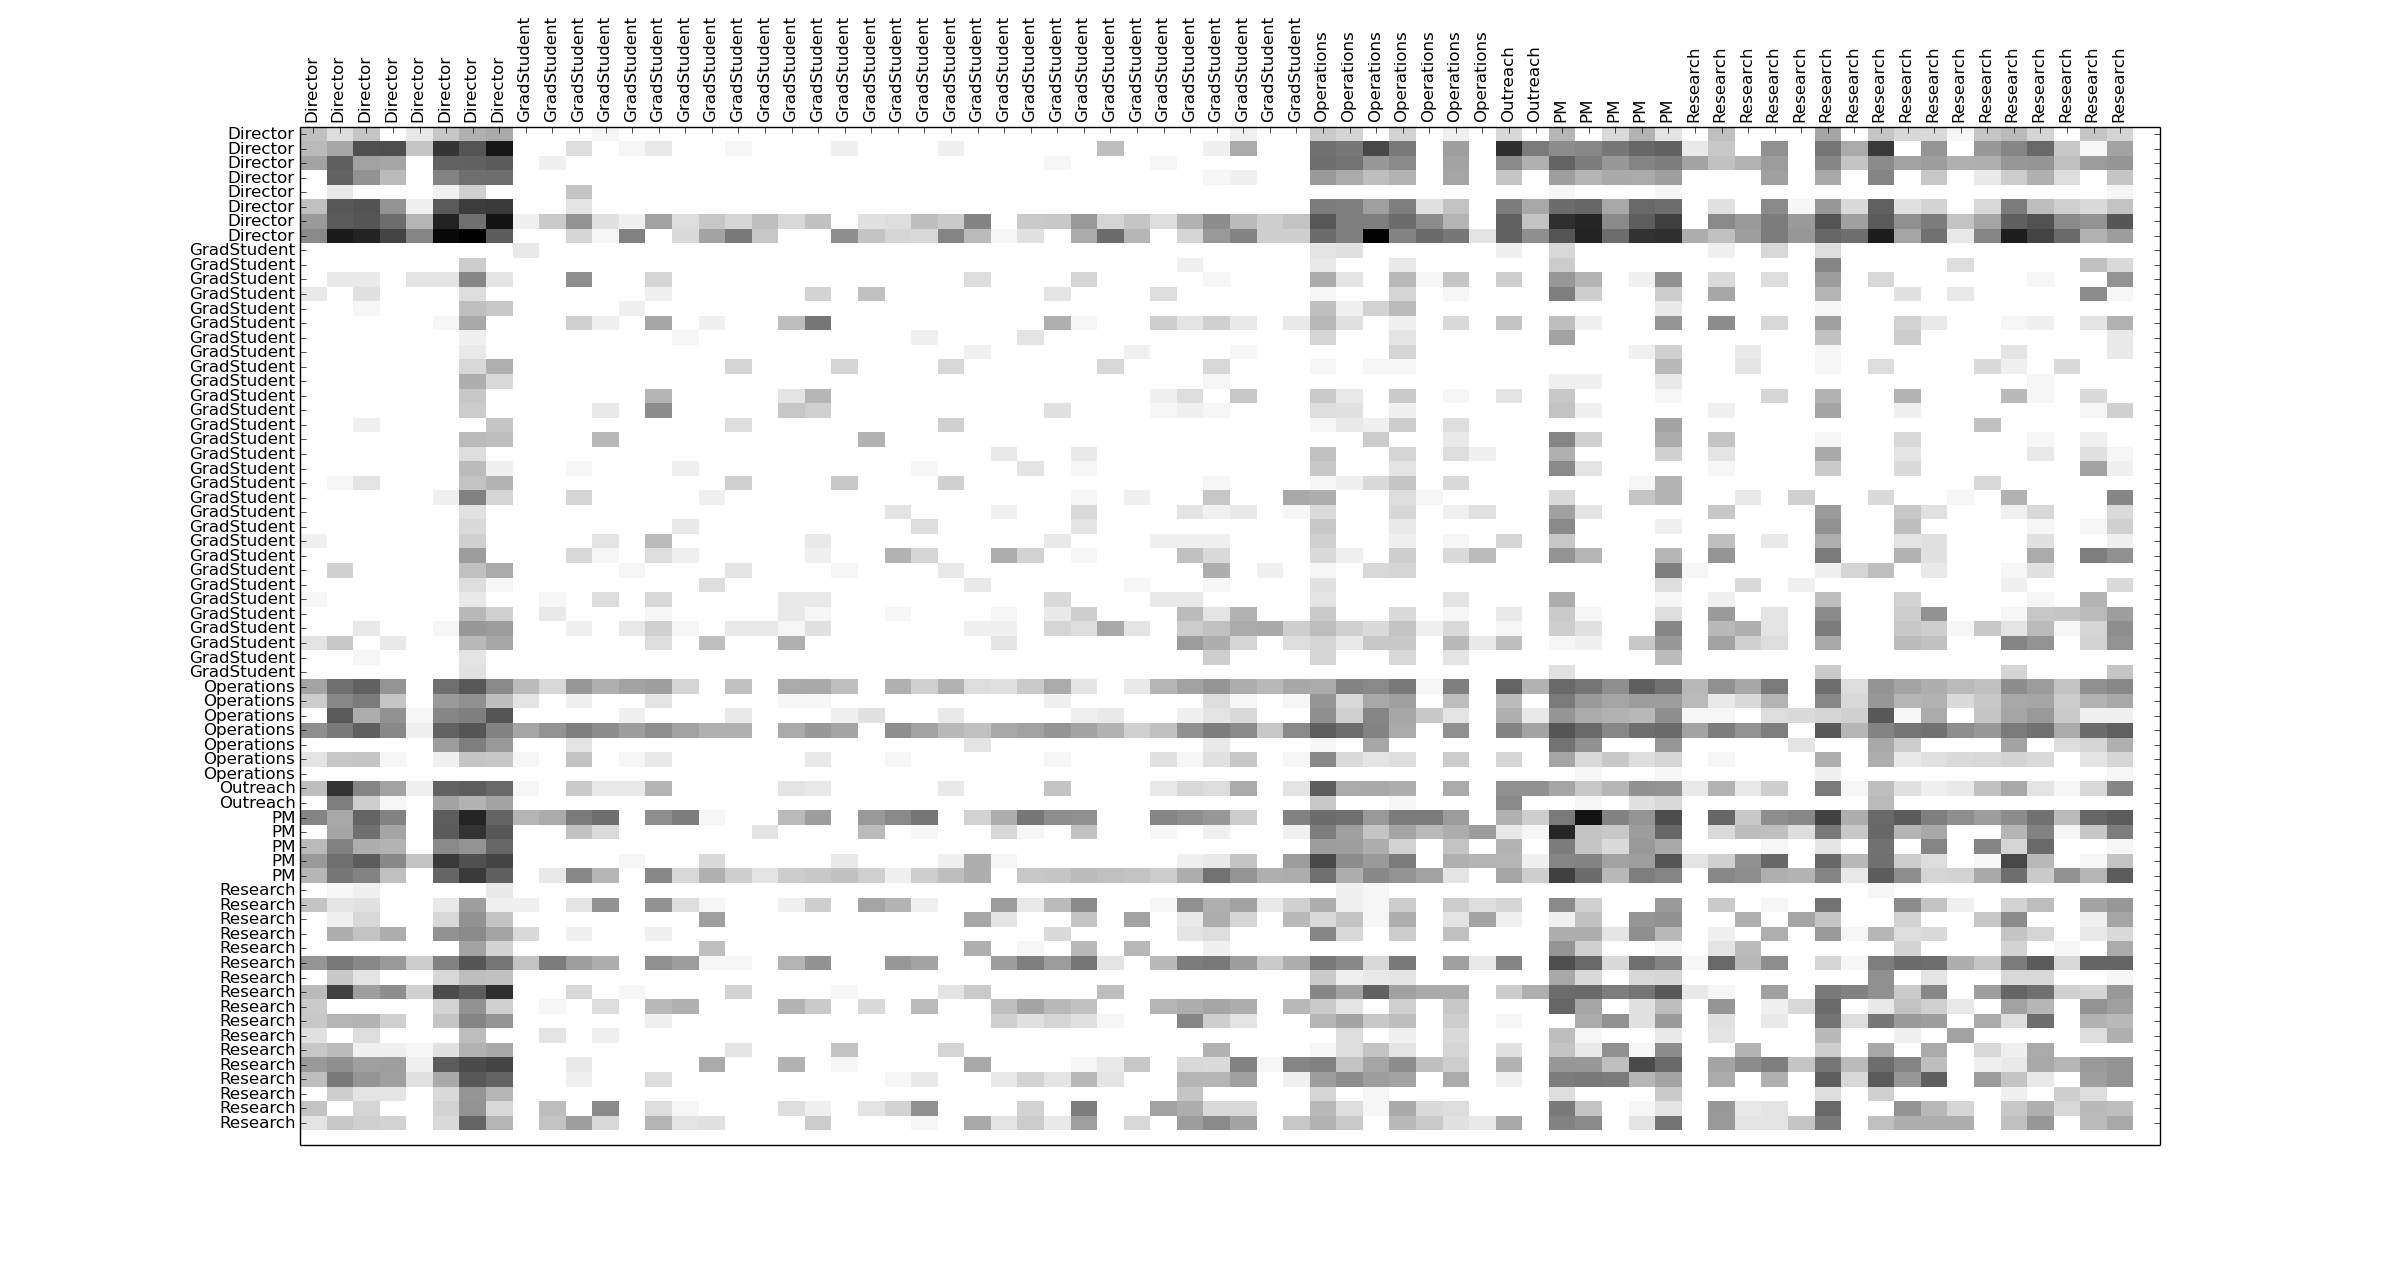
\includegraphics[width=0.5\textwidth]{adj_matrix}
        \caption{Adjacency matrix representing the social connections of the workplace.}
        \label{fig:var_imp}
\end{figure}
\item Highlight top 3 social-based features
\end{itemize}

\section{Analysis}

\begin{itemize}
\item Because of low sample size but high number of features, selected random forest as classification method
    \begin{itemize}
    \item Describe Random Trees
    \begin{figure}[H]
    \centering
        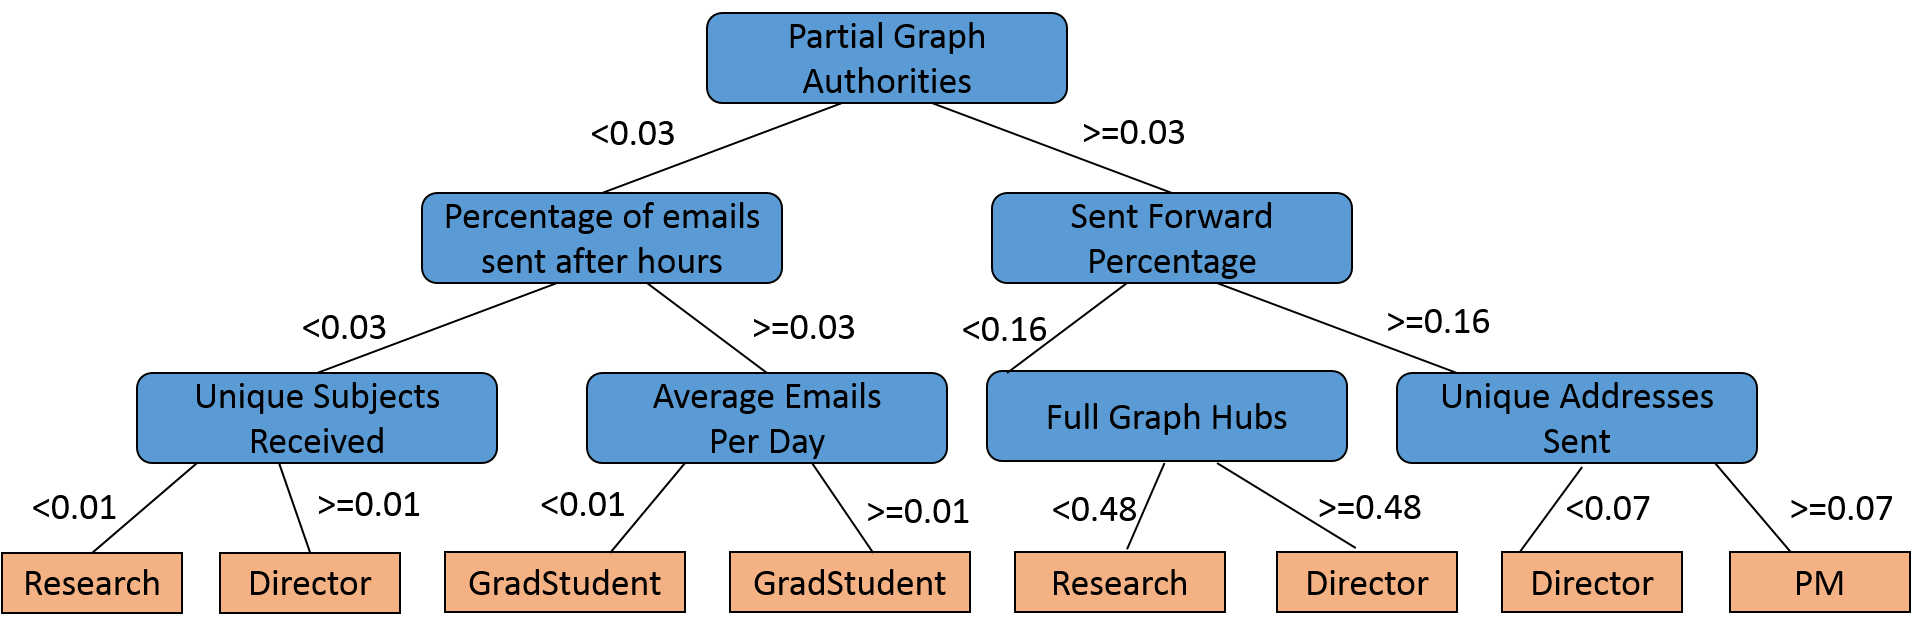
\includegraphics[width=0.5\textwidth]{3_level_tree}
        \caption{Example random tree of depth 3.}
        \label{fig:ex_tree}
\end{figure}

    \item Random Forests use bootstrap AND bagging on random trees - use random components, create many, very deep trees, take a vote to classify
    \item Biggest advantage: doesn't overfit
    \end{itemize}

\item Used information gain as feature selection method.  Describe this process

\begin{table}[H]
\centering
\caption{Top 20 features ranked by the information gain method.  Note that out of the to 20, there are 12 traffic-based features and 8 that are graph-based.}
\label{tab:ranked_feats}
\begin{tabular}{lll}
\cline{1-1}
\multicolumn{1}{|l|}{Feature}                & Type         & Ranker\\ \cline{1-1}
unique\_subjects\_received                   & Traffic      & 0.728 \\
total\_received\_signed                      & Traffic      & 0.728 \\
rec\_fw                                      & Traffic      & 0.719 \\
fg\_hubs                                     & Graph        & 0.589 \\
pg\_communicability\_centrality              & Graph        & 0.554 \\
pg\_communicability\_betweenness\_cent       & Graph        & 0.554 \\
rec\_cc                                      & Traffic      & 0.507 \\
rec\_fw\_perc                                & Traffic      & 0.503 \\
pg\_degree\_centrality                       & Graph        & 0.492 \\
pg\_pagerank                                 & Graph        & 0.492 \\
pg\_current\_flow\_closeness\_centrality     & Graph        & 0.492 \\
avg\_rec\_per\_day                           & Traffic      & 0.489 \\
avg\_emails\_per\_day                        & Traffic      & 0.479 \\
pg\_avg\_shortest\_paths                     & Graph        & 0.476 \\
pg\_colseness\_centrality                    & Graph        & 0.476 \\
unique\_addresses\_received\_signed          & Traffic      & 0.457 \\
sent\_cc                                     & Traffic      & 0.43  \\
rec\_re                                      & Traffic      & 0.43  \\
avg\_sent\_per\_day                          & Traffic      & 0.404
\end{tabular}
\end{table}

\item Manually looked at feature breakdown compared to classes

\begin{figure}[H]
    \centering
        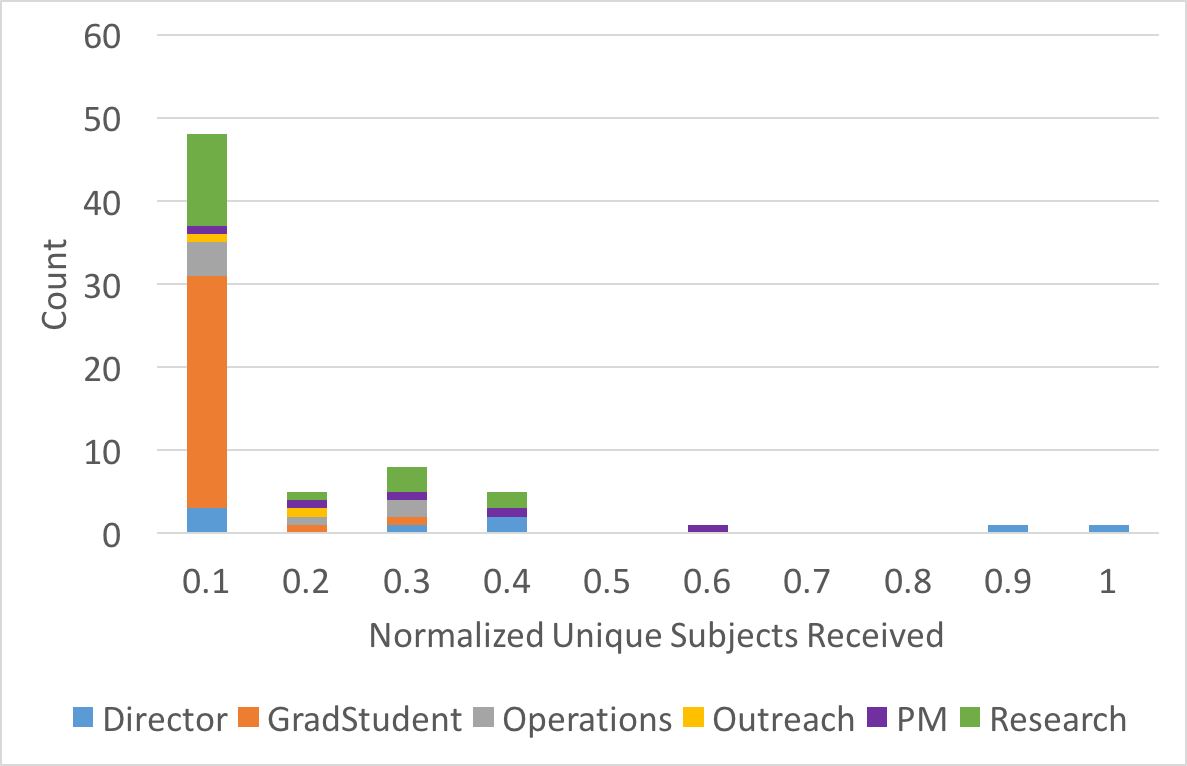
\includegraphics[width=0.4\textwidth]{Unique_subjects_rec_hist}
        \caption{Histogram of unique subjects received by job title.}
        \label{fig:traffic_ex_hist}
\end{figure}


\begin{figure}[H]
    \centering
        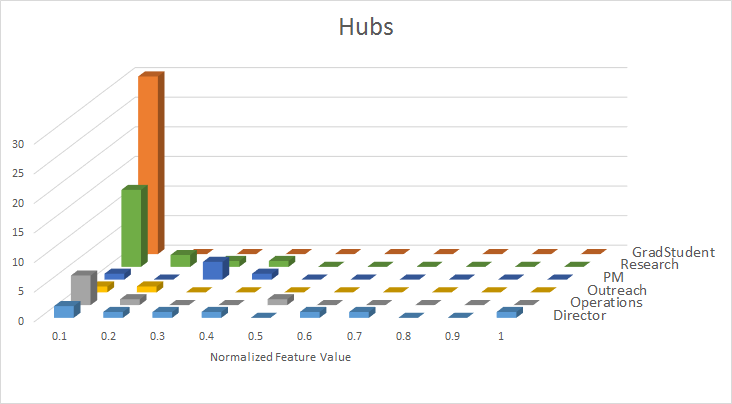
\includegraphics[width=0.4\textwidth]{Hubs_hist}
        \caption{Histogram of hubs from social graph by job title.}
        \label{fig:social_ex_hist}
\end{figure}

\item Looked at prediction accuracy vs. number of features

\begin{figure}[H]
    \centering
        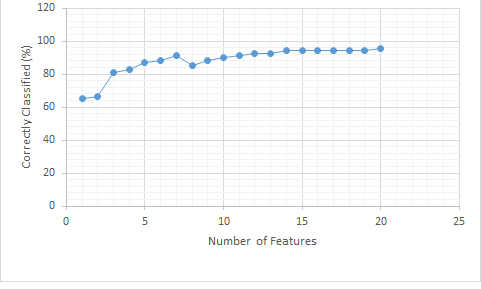
\includegraphics[width=0.4\textwidth]{FeatureAnalysis}
        \caption{Prediction accuracy compared to number of features used for analysis.}
        \label{fig:feat_analysis}
\end{figure}

\end{itemize}

\section{Results}
\subsection{Classification Results}
\begin{itemize}

\item Explain splitting process (train on random \% of emails, test on the rest)
\item Looked into optimal train/test split:

\begin{figure}[H]
    \centering
        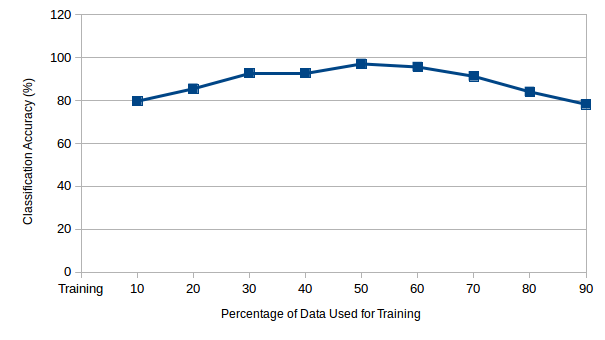
\includegraphics[width=0.4\textwidth]{SplitAnalysis}
        \caption{Prediction accuracy compared to percentage of data used for training.}
        \label{fig:split_analysis}
\end{figure}

\item Based on the above result, I used a 50/50 split for the analysis of the classifier.

\item Classification Results
\item Assumption: employees with the same title exhibit
\begin{figure}[H]
    \centering
        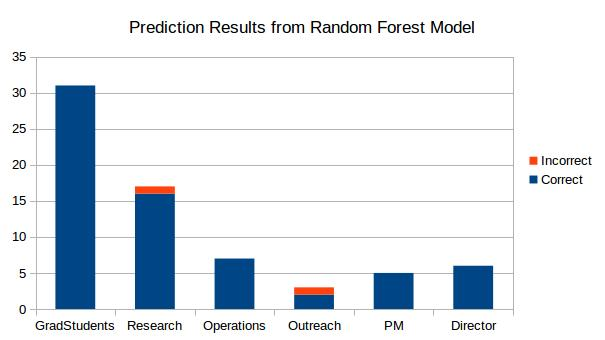
\includegraphics[width=0.5\textwidth]{Prediction_50_50_RF}
        \caption{Prediction accuracy for test set using Random Forest model.  Data was split such that 50\% was used as training data and 50\% was used as testing data.}
        \label{fig:result_hist}

\end{figure}

\item Even the errors are explainable (not much data on Outreach.  The researcher that was misclassified was mislabelled as a graduate student, and this person is a post-doc.
\item Both misclassifications were second-ring 

\subsection{Hierarchy Analysis}
    \begin{itemize}
    \item Only 57.58\% of employees communicate most frequently with their director from the organization chart.
    \item 72.73\% of graduate students and researchers communicate most frequently with their primary program manager.
    \end{itemize}
\item Many of the discrepancies make sense to those of us with insider knowledge and reflect formal choices made in generating the org chart

\end{itemize}



\section{Conclusions and Future Work}
\begin{itemize}
\item Presented new dataset that was carefully cleaned with inside knowledge and has accurate labels.
\item Random Forests are shown to be powerful classifiers for this data.  They classified with high accuracy
\item Used both traffic-based and graph features helped improve accuracy
\item Acknowledge we are testing back on ourselves, randomness in email splitting process
\item From our intimate knowledge of the workings of the lab, we know that hierarchy discrepancies can be explained by multiple projects, directors/PMs working in different offices, etc.
\item Do more things with dataset
\item Evaluate methods on Enron/Hillary Clinton's emails and compare which features are consistent predictors
\end{itemize}

\bibliographystyle{named}
\bibliography{bib}


\end{document}